\chapter{SSLStrip NTP}

\label{sec:sslstrip-ntp}

\begin{figure}[H]
  \caption{Attaque SSLStrip NTP (diagramme Dia)}
  \fbox{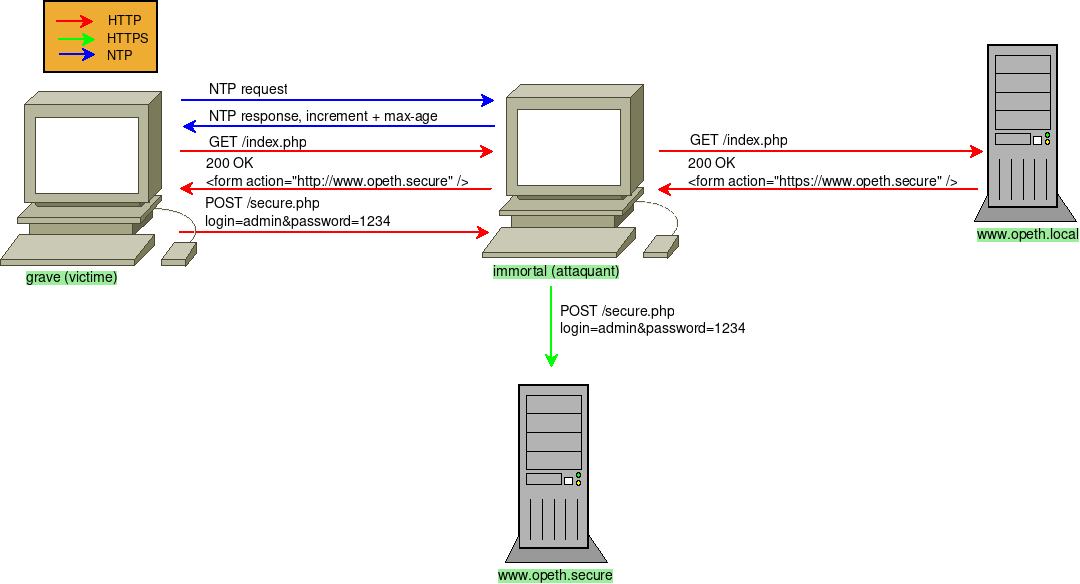
\includegraphics[width=\textwidth]{../medias/sslstrip-ntp/attack.png}}
\end{figure}

\section{Description de l'attaque}

Cette nouvelle amélioration de l'attaque SSLStrip a été présentée lors de la BlackHat Europe par Jose Selvi. Celle-ci utilise le protocole NTP afin de contourner la sécurité offerte par HSTS.

L'attaque SSLStrip originale n'est en effet plus possible lorsque l'on essaye de "stripper" les URL d'une page web d'un domaine qui a été protégé ultérieurement par HTTP Strict Transport Security. Le mécanisme HSTS va obliger le client à se connecter à l'URL que l'on cherche à stripper en HTTPS pendant un certain laps de temps (défini par le serveur), rendant l'attaque complètement inefficace.

Le protocole NTP (Network Time Protocol) permet de synchroniser l'horloge d'un équipement informatique avec un serveur NTP. Il s'agit d'un protocole sans états basé sur UDP et absolument pas sécurisé. L'attaque présentée par Jose Selvi consiste à usurper les requêtes NTP pour renvoyer une date erronée au client, et ainsi faire expirer les entrées HSTS. Pour réaliser cela, l'auteur se base sur un outil Python appelé Delorean, qui se comporte comme un serveur NTP et pour lequel on peut définir la date de réponse.

Une fois que l'horloge du client a été compromise et le HSTS du domaine expiré, il est possible d'utiliser l'attaque SSLStrip originale afin de stripper les URL des pages web, même pour les domaines censés être protégés par HSTS.

\section{Notre attaque}

Dans ce projet de TER, nous avons eu à réaliser une preuve de concept de cette attaque. Voici les détails de notre implémentation.

\subsection{Mise en place de l'environnement}

Pour résoudre les différents domaines, nous utilisons le fichier \path{/etc/hosts} de chaque machine.

\subsubsection{Configuration de la machine serveur - opeth}

Pour cette attaque, nous avons ajouté un serveur NTP légitime sur la machine \textbf{opeth}, à travers l'outil ntpd. La configuration de base était suffisante pour notre démonstration. À noter que dans la réalité, le serveur NTP aurait été probablement sur une machine différente.

Concernant le serveur web NGINX, celui-ci utilise les deux domaines \path{www.opeth.local} et \path{www.opeth.secure}. Le premier est accédé en HTTP alors que le second en HTTPS et protégé grâce à HSTS.

\subsubsection{Configuration de la machine cliente - grave}

Il a fallut utiliser un client NTP sur cette machine pour cette attaque. Nous utilisons donc sntpc (Simple NTP Client), que l'on lance au démarrage de la machine et que l'on configure pour effectuer ses requêtes vers \textbf{opeth} de manière régulière (toutes les secondes pour les besoins de la démonstration).


\subsubsection{Configuration de la machine attaquante - immortal}

C'est sur cette machine que se trouve la preuve de concept de l'attaque. Nous avons également utilisé le script Delorean \cite{delorean} comme décrit dans le papier de l'attaque afin d'usurper les requêtes NTP de la machine grave. L'attaque se lance grâce au script \path{/mnt/host/attack.sh} :

\inputminted[bgcolor=lbcolor, breaklines]{bash}{../sslstrip-ntp/immortal/attack.sh}

Nous commençons par rediriger les requêtes HTTP sur le port de notre proxy, puis les requêtes NTP vers le port de Delorean. Nous calculons ensuite le temps d'expiration des entrées HSTS à l'aide de l'outil curl. Finalement, nous lançons le serveur Delorean ainsi que notre proxy implémentant l'attaque SSLStrip.

\subsection{Démonstration}

Dans cette partie, nous allons illustrer l'attaque SSLStrip NTP dans l'environnement que nous avons mis en place. Pour lancer l'environnement de test, il suffit de lancer qemunet de la manière suivante :

\begin{minted}{bash}
./qemunet/qemunet.sh -x -S sslstrip-ntp
\end{minted}

À partir de là, les trois machines sont lancées.

\subsubsection{Étape 1 : avant l'attaque}

Lorsque l'attaque n'est pas encore lancée, nous pouvons voir sur la machine grave que tout se passe normalement et que la requête POST passe bien en HTTPS ; immortal est donc incapable de voir les identifiants envoyés :

\begin{figure}[H]
  \caption{Attaque SSLStrip NTP (avant l'attaque)}
  \fbox{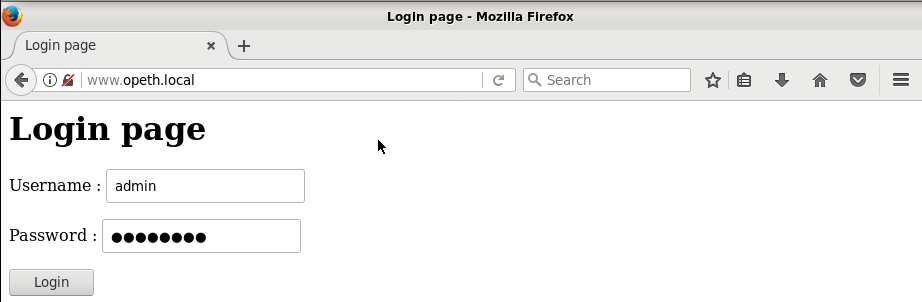
\includegraphics[width=\textwidth]{../medias/sslstrip-ntp/screen1.png}}
\end{figure}


L'encadré rouge ci-dessous montre bien que le POST est effectué en HTTPS, sur le domaine \path{www.opeth.secure}. Lorsque nous affichons le code source de la page, nous obtenons :

\begin{figure}[H]
  \caption{Code source de la page (avant l'attaque)}
  \fbox{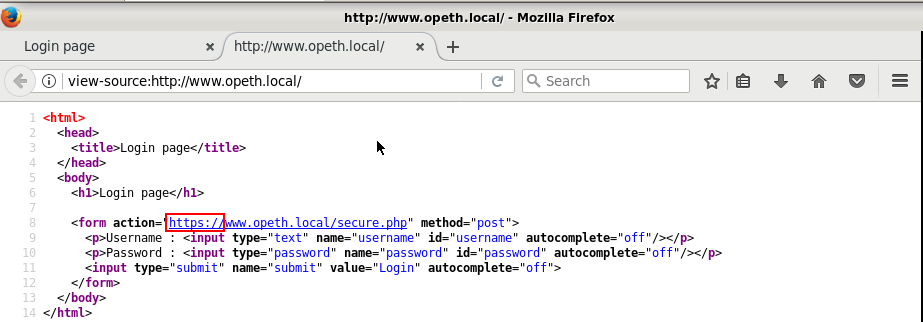
\includegraphics[width=\textwidth]{../medias/sslstrip-ntp/screen2.png}}
\end{figure}

Nous arrivons alors sur le domaine \path{www.opeth.secure} en HTTPS : immortal n'a pas pût voir nos échanges sur cette page sécurisée comme le montre la figure ci-dessous.

\begin{figure}[H]
  \caption{La connexion se fait bien en HTTPS}
  \fbox{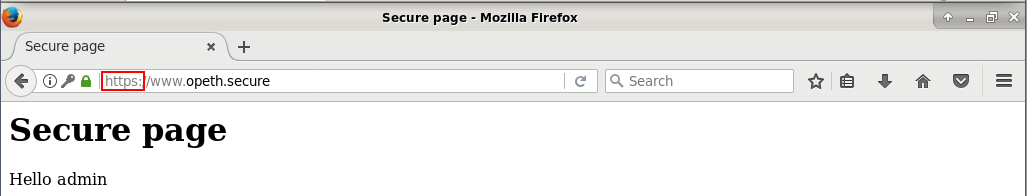
\includegraphics[width=\textwidth]{../medias/sslstrip-ntp/screen3.png}}
\end{figure}

\subsubsection{Étape 2 : pendant l'attaque}

Lorsque l'attaque est en cours et quand le client réalisera une requête NTP, celle-ci va être redirigée vers Delorean qui répondra avec une date permettant de faire expirer son entrée HSTS. Ensuite, quand la machine grave visitera la page non-sécurisée \path{www.opeth.local}, tous les liens HTTPS vers \path{www.opeth.secure} seront strippés.

Ici on voit dans le code source de la page que notre proxy a remplacé les liens \path{https://} par \path{http://}.

\begin{figure}[H]
  \caption{Code source de la page (pendant l'attaque)}
  \fbox{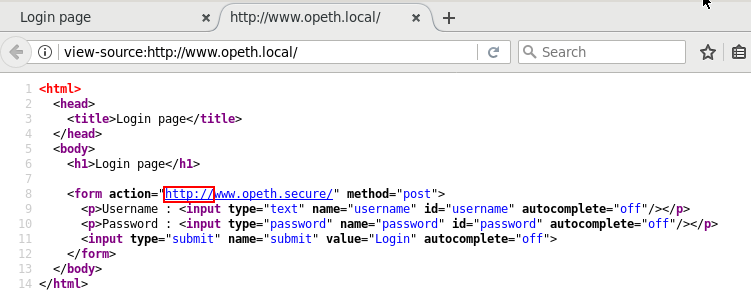
\includegraphics[width=\textwidth]{../medias/sslstrip-ntp/screen5.png}}
\end{figure}

Nous constatons que nous arrivons sur le domaine \path{www.opeth.secure} en HTTP : notre navigation n'est pas sécurisée !

\begin{figure}[H]
  \fbox{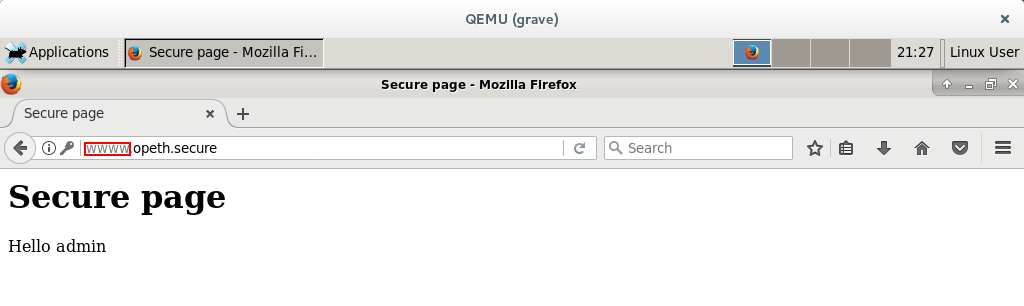
\includegraphics[width=\textwidth]{../medias/sslstrip-ntp/screen6.png}}
\end{figure}

La machine immortal a été capable de capturer non seulement les identifiants du formulaire, mais également le cookie de session alors que le domaine était protégé par HSTS :

\begin{figure}[H]
  \fbox{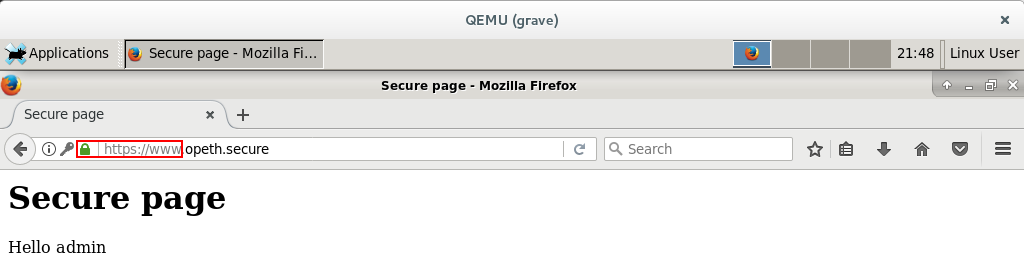
\includegraphics[width=\textwidth]{../medias/sslstrip-ntp/screen7.png}}
\end{figure}

Le script complet de l'attaque peut être consulté à l'annexe \ref{appendix:sslstrip-ntp}.

\section{Limitations de notre attaque}

Dans cette attaque, nous supposons que le client effectue des requêtes NTP. Ceci n'est en fait pas toujours le cas, et il arrive que des clients n'utilisent pas NTP pour mettre leur horloge à jour.

De plus, ici notre attaque fonctionne relativement rapidement car notre client a été configuré pour effectuer ses requêtes toutes les secondes. En pratique, l'attente d'une requête NTP peut être beaucoup plus longue et est souvent de l'ordre de plusieurs heures.

Une autre supposition que nous avons faite mais qui n'est peut être pas possible en réalité est que nous sommes sur le chemin entre le client et le serveur NTP. Suivant à quel endroit l'attaquant a réussi à se placer en homme du milieu, l'attaque pourrait ne pas être possible.

Ce script possède également les même limitations que celui sur \hyperref[sec:sslstrip]{SSLStrip}.
